\documentclass[border={5cm 0.25cm 5cm 0.25cm}]{standalone}
\usepackage[utf8]{inputenc}
\usepackage{tikz}
\usepackage{lipsum}
\usepackage{mwe}
\usetikzlibrary{decorations.pathreplacing,matrix}
\usetikzlibrary{positioning,automata,arrows,shapes.misc}
\begin{document}
\hspace{1cm}
\centering

\begin{minipage}[t]{1.0\linewidth}%

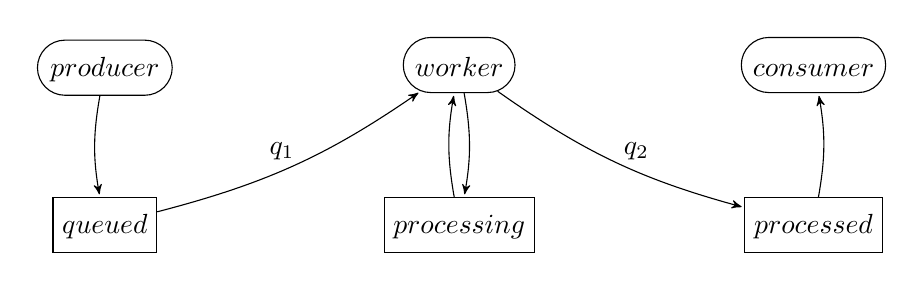
\begin{tikzpicture}[->,>=stealth',shorten >=1pt,auto,anchor=base,node distance=2cm,text height=8pt,minimum height=7mm]

\matrix [matrix of math nodes,
column sep={2.25cm,between origins},
row sep={1cm,between origins},
nodes={minimum height=7mm}]
{
|(producer)[draw,rounded rectangle]| producer & &
|(worker)[draw,rounded rectangle]| worker & &
|(consumer)[draw,rounded rectangle]| consumer  \\
 & |(q1)| q_1 & & |(q2)| q_2 & \\
|(queued)[draw,rectangle]| queued & &
|(processing)[draw,rectangle]| processing & &
 |(processed)[draw,rectangle]| processed \\
};

  \path (producer) [out=-10,in=190,relative]  edge node {} (queued)
        (queued)                              edge node {} (worker)
        (processing)[out=10,in=170,relative]  edge node {} (worker)
        (worker)                              edge node {} (processing)
        (worker)    [out=-10,in=190,relative] edge node {} (processed)
        (processed)                           edge node {} (consumer);

\end{tikzpicture}

\end{minipage}
\end{document}
